%! Author = danielmendes
%! Date = 29.11.24

\chapter{Indizes}\label{ch:indexes}

Das folgende Kapitel befasst sich mit der Indexierung und den damit verbundenen Performance-Optimierungen, die näher erläutert werden.
Zunächst werden einige Grundlagen betrachtet.
Anschließend werden die verschiedenen Arten von Indizes näher erklärt und unterschiedliche Benchmarks mit ihnen durchgeführt.
Im letzten Schritt werden die Ergebnisse analysiert, um festzustellen, welche Verwendung der Indizes am besten funktioniert.

\section{Grundlagen}\label{sec:indexing-grundlagen}

Indizes sind Datenstrukturen, die von Speicher-Engines (engl.\ storage engines) verwendet werden, um Zeilen schneller zu finden.
Die Storage-Engine ist eine Kernkomponente eines Datenbankmanagementsystems, die für die Speicherung und Verwaltung der Daten verantwortlich ist.
Verschiedene Storage-Engines unterscheiden sich hinsichtlich ihrer Indexfunktionalität sowie der Unterstützung von Transaktionen und Sperrmechanismen.
Im weiteren Verlauf werden verschiedene Indextypen vorgestellt, die nicht von allen Engines unterstützt werden.

Mit zunehmender Größe der Datenbank wird das Scannen aller Tupel immer aufwendiger, weshalb Indizes eine zentrale Rolle für die Datenbank-Performance spielen.
Weniger ausgelastete Datenbanken können ohne ordnungsgemäße Indizes gut funktionieren, aber die Leistung kann rapide sinken, wenn die Datenmenge wächst.
Wenn ein solches Problem auftritt, ist die Index-Optimierung oft der effektivste Weg, um die Abfrageleistung schnell zu verbessern.
Um wirklich optimale Indizes zu erstellen, ist es häufig notwendig, Abfragen umzuschreiben.
Besonders nützlich sind Indizes bei Abfragen, die Joins zwischen mehreren Tabellen enthalten, da sie ermöglichen, die Anzahl der zu prüfenden Tupel erheblich zu reduzieren, wenn eine einschränkende Bedingung vorliegt.

Um die Funktionsweise eines Indexes anschaulicher zu erklären, wird als Beispiel ein wissenschaftliches Fachbuch betrachtet (vgl.\ \cite[S. 147]{schwartz2012high}).
Am Ende dieser Bücher gibt es meist ein Stichwortverzeichnis oder Register.
Dieses Register besteht aus einer alphabetisch geordneten Liste von Begriffen, Themen und Stichworten.
Möchte man einen Begriff nachschlagen, sucht man ihn im Stichwortverzeichnis und erhält die Seitenzahlen, auf denen er vorkommt.
In DBMS verwendet die Storage-Engine Indizes auf eine ähnliche Weise.
Sie durchsucht die Datenstruktur des Indexes nach einem Wert.
Und wenn ein Treffer gefunden wird, kann die Engine die Zeilen ermitteln, die den Treffer enthalten.
Das folgendes Beispiel veranschaulicht dies:

\begin{lstlisting}[language=SQL]
SELECT NAME FROM KUNDEN WHERE KUNDEN_ID = 7;
\end{lstlisting}
\vspace{-4pt}

Angenommen, es existiert ein Index auf der Spalte \texttt{KUNDEN\_ID}, dann wird MySQL diesen verwenden, um Zeilen zu finden, bei denen die \texttt{KUNDEN\_ID} den Wert 7 hat.
Ein Index kann aber nicht nur die Werte einer einzelnen Spalte enthalten, sondern auch mehrere Spalten einer Tabelle umfassen.
Bei mehrspaltigen Indizes spielt die Reihenfolge der Spalten im Index eine entscheidende Rolle.
Außerdem ist der Zugriff auf nicht alle Spalten bedingungslos effizient, da MySQL nur auf das linkeste Präfix des Indexes zugreifen kann.
Wenn man nur das zweite Attribut eines Indexes angibt, ohne das erste zu referenzieren, kann der Index nicht direkt verwendet werden.
Es ist wichtig zu beachten, dass ein Index, der über zwei Spalten definiert ist, nicht mit zwei getrennten einspaltigen Indizes gleichzusetzen ist.
In diesem Fall können Abfragen nur auf einer der beiden Spalten basieren, was zu schlechterer Performance führt, wenn beide Spalten gleichzeitig abgefragt werden.

Um zu verstehen, wie man Indizes für eine Datenbank auswählt, ist es wichtig zu wissen, welcher Teil der Abfrage am meisten Zeit in Anspruch nimmt (\cite[S. 350--353]{garcia2008database}).
Das Datenbanksystem verteilt die Tupel einer Relation üblicherweise auf viele Festplattenseiten.
Um die Werte eines Tupels zu prüfen, muss die gesamte Seite, auch Block genannt, in den Hauptspeicher geladen werden.
Dabei erfordert es nahezu gleich viel Zeit, alle Tupel einer Seite zu prüfen, anstatt nur ein einzelnes.
Aufgrund dieser Tatsache kann die Entscheidung, ob für ein bestimmtes Attribut ein Index definiert werden soll, von drei Faktoren abhängig gemacht werden.
Erstens ist ein Index besonders nützlich, wenn Abfragen häufig auf ein bestimmtes Attribut zugreifen.
Zweitens kann ein Index sinnvoll sein, wenn es nur wenige Tupel für einen bestimmten Wert des Attributs gibt, da dies den Festplattenzugriff bei einer Abfrage reduziert.
Und der letzte Fall betrifft Situation, in denen Tupel nach einem Attribut geclustert sind.
Da die Werte des Attributs aufeinanderfolgender gespeichert sind, müssen durch einen Index weniger Datenblöcke geladenen werden.

Trotz dieser Faktoren müssen Entwickler bei der Auswahl von Schlüsseln und Indizes einen Tradeoff abwägen.
Es gibt dabei zwei Faktoren, die die Entscheidung beeinflussen.
Zum einen kann ein Index auf einem Attribut Abfragen mit diesem Attribut erheblich beschleunigen.
Zum anderen erschwert jeder Index Einfügungen, Löschungen und Aktualisierungen, da diese mehr Zeit und Aufwand erfordern.
Dennoch kann ein Index auf ein häufig verändertes Attribut die Leistung verbessern, da einige Modifikationen zunächst eine Datenbankabfrage erfordern.
Im Kapitel \nameref{ch:partitions} wird dieses Thema erneut behandelt

Zur Entscheidungsfindung anhand einer Berechnung wird die folgende Tabelle verwendet (abgeändertes Beispiel aus~\cite[S. 355--357]{garcia2008database}):
\vspace{-4pt}
\begin{lstlisting}
Fakten(Id, Bestelldatum, Artikel_Id, Kunden_Id, ...)
\end{lstlisting}
\vspace{-8pt}

Der Schlüssel der Faktentabelle ist die Spalte \texttt{Id} und für die \texttt{Artikel\_Id} sowie die \texttt{Kunden\_Id} werden eigene Indizes erstellt, sodass insgesamt drei Indizes vorhanden sind.
Als Nächstes werden Befehle benötigt, bei denen die Indizes benutzt werden (siehe~\ref{lst:indexing:fakten-select-insert-queries}).
In der ersten Zeile wird nur der Kundenindex verwendet und in der zweiten nur der Artikelindex.

\vspace{-12pt}
\begin{lstlisting}[language=SQL,caption=Select-Queries für die Faktentabelle,label={lst:indexing:fakten-select-insert-queries}]
SELECT Bestelldatum, Artikel_Id FROM Fakten WHERE Kunden_Id = k;
SELECT Bestelldatum, Kunden_Id FROM Fakten WHERE Artikel_Id = a;
\end{lstlisting}
\vspace{-8pt}

Damit berechnet werden kann, ob es sinnvoll ist, die Indizes zu erstellen, müssen bestimmte Voraussetzungen festgelegt werden.
Zuallererst wird davon ausgegangen, dass die Faktentabelle 10 Datenblöcke belegt und im Durchschnitt jeder Kunde 3 Artikel kauft, während ein Artikel von 3 Kunden gekauft wird.
Die Tupel für einen bestimmten Kunden oder Artikel sind gleichmäßig über die 10 Seiten verteilt.
Trotzdem sind mit einem Index nur 3 Festplattenzugriffe erforderlich, um die durchschnittlich 3 Tupel für einen Kunden oder Artikel zu finden.
Um die Seite des Indexes zu lesen, ist ein Festplattenzugriff erforderlich und ein weiterer, um die modifizierte Seite zurückzuschreiben, falls eine Indexseite geändert werden muss.
Ohne Index sind 10 Festplattenzugriffe zum Lesen und zwei Festplattenzugriffe zum Schreiben erforderlich.
Unter diesen Bedingungen ergibt sich die folgende Kostentabelle:

\vspace{-18pt}
\begin{table}[H]
    \centering
    \setlength{\arrayrulewidth}{0.4mm}
    \[
        \begin{array}{r|c c c c}
            \textbf{Aktion} & \textbf{Kein Index} & \textbf{Kunden Index} & \textbf{Artikel Index} & \textbf{Beide Indizes} \\ \hline
            Q_1 & 10 & 4 & 10 & 4 \\
            Q_2 & 10 & 10 & 4 & 4 \\
            I   & 2  & 4  & 4  & 6 \\ \hline
            \textbf{Durchschnitt} & 2 + 8p_1 + 8p_2 & 4 + 6p_2 & 4 + 6p_1 & 6-2p_1-2p_2 \\
        \end{array}
    \]
    \vspace{-5pt}
    \caption[Performance-Vergleich]{Kosten der unterschiedlichen Queries in Abhängigkeit der Indizes}
    \label{tab:performance-queries}
\end{table}
\vspace{-25pt}

Unter der Annahme, dass die erste Abfrage p1 und die zweite p2 der Zeit beansprucht, ergibt sich für I ein Anteil von 1 – p1 – p2.
Damit kann der Durchschnitt für den Kundenindex wird wie folgt berechnet (siehe letzte Zeile aus~\ref{tab:performance-queries}):
\[
    4p_{1} + 10p_{2} + 4 \cdot (1 - p_{1} - p_{2}) = 4p_{1} + 10p_{2} + 4 - 4p_{1} - 4p_{2} = 4 + 6p_{2}
\]

Abhängig von den Werten für p1 und p2 kann jede der vier Optionen die geringsten Kosten für die drei Operationen verursachen.
Zum Beispiel, wenn p1 = p2 = 0,1, dann ist der Ausdruck 2 + 8p1 + 8p2 am kleinsten, sodass keine Indizes bevorzugt werden würden.
Damit wurde gezeigt, dass es sinnvoll ist, keinen Index zu verwenden, wenn überwiegend Einfügungen durchgeführt werden und nur sehr wenige Abfragen anfallen.
Intuitiv gilt, dass bei vielen Abfragen und einer ungefähr gleichen Häufigkeit von Abfragen, die Artikel und Kunden angeben, beide Indizes vorteilhaft sind.
Wird hingegen nur ein Typ von Abfrage häufig genutzt, sollte nur der Index definiert werden, der bei dieser Abfrageart hilft.

Um die Verantwortung für die Wahl der Indizes vom Datenbankdesigner zu übernehmen, wurden zahlreiche Tools entwickelt.
Dabei optimiert das System sich selbst oder dem Entwickler werden zumindest Empfehlungen für sinnvolle Entscheidungen gegeben.
Ein bewährter Ansatz zur Auswahl von Indizes ist das sogenannte Greedy-Verfahren (\cite[S. 824]{garcia2008database}), bei dem zunächst ohne ausgewählte Indizes der Nutzen jedes Kandidaten-Index bewertet wird.
Wenn es einen Index mit positivem Nutzen gibt, wird dieser ausgewählt und anschließend wird eine Neubewertung ausgeführt, wobei davon ausgegangen wird, dass der zuvor ausgewählte Index bereits verfügbar ist.
Dieser Prozess wird so lange wiederholt, bis es keinen Kandidaten-Index mit positivem Nutzen mehr gibt.

\section{B-Baum-Index}\label{sec:indexing-b-baum-index}

Der erste zu betrachtende Indextyp ist der B-Baum-Index (engl.\ B-Tree Index), der auf einer speziellen Baum-Datenstruktur basiert.
Diese Struktur wird von den meisten MySQL-Storage-Engines unterstützt.
Außerdem verwendet ihn MySQL standardmäßig für die Primary Keys (\cite{mysql_primary_key}).
Die Implementierung und Nutzung des B-Baum-Indexes kann je nach verwendeter Storage-Engine variieren.

Das Grundprinzip eines B-Baums ist, dass alle Werte in einer bestimmten Reihenfolge gespeichert werden und jede Blattseite den gleichen Abstand zum Wurzelknoten hat.

\begin{quote}
    \enquote{The height of a B+ tree depends on the number of data entries and the size of index entries.} (\cite[S. 358]{ramakrishnan2002database})
\end{quote}

Ein B-Baum-Index beschleunigt den Datenzugriff, da die Storage-Engine nicht die gesamte Tabelle durchsuchen muss, um die gewünschten Daten zu finden.
Stattdessen beginnt die Suche beim Wurzelknoten.
Die Slots im Wurzelknoten enthalten Zeiger auf Kindknoten und die Storage-Engine folgt diesen Zeigern.
Der richtige Zeiger wird durch Vergleich der Werte in den Knoten-Seiten (engl.\ node pages) ermittelt, die die oberen und unteren Grenzen der Werte in den Kindknoten definieren.
Letztlich stellt die Storage-Engine fest, ob der gewünschte Wert existiert oder ob sie erfolgreich eine Blatt (engl.\ leaf page) erreicht.

\vspace{-8pt}
\begin{figure}[H]
    \centering
    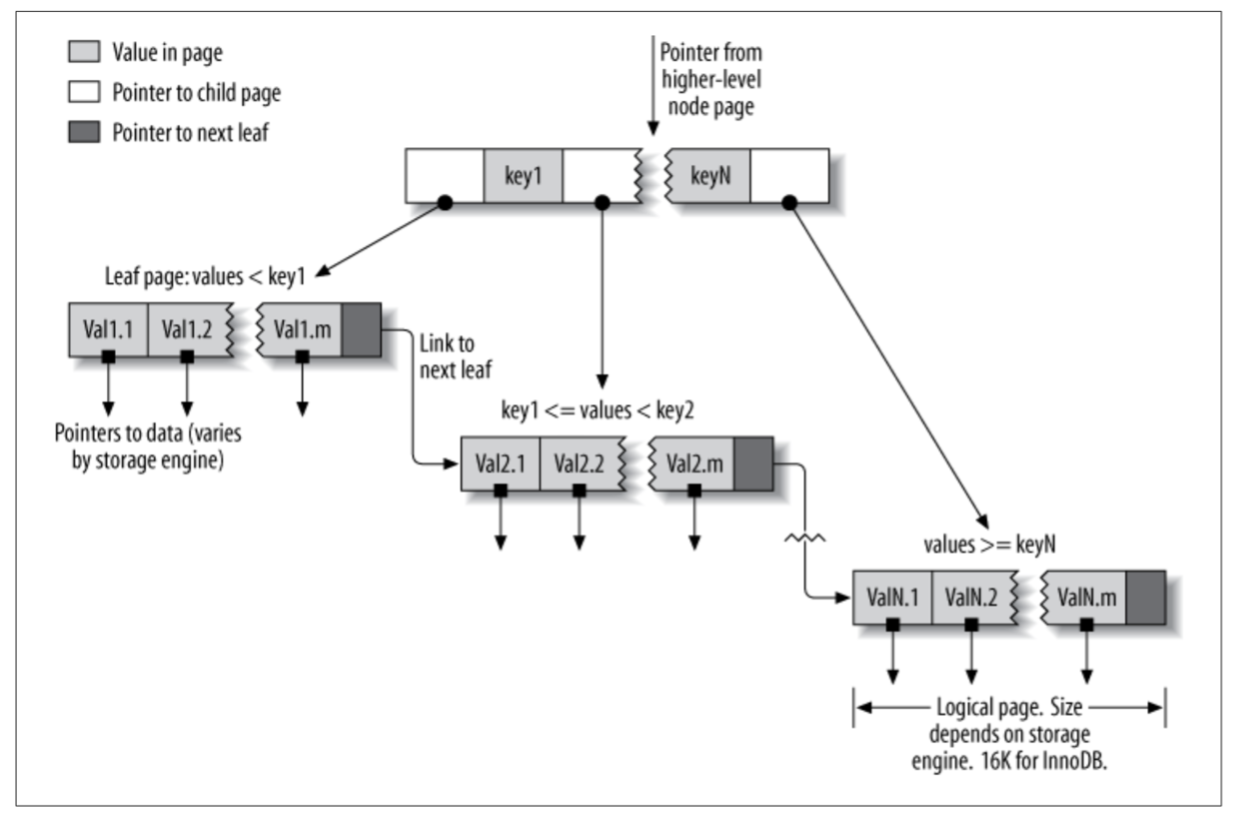
\includegraphics[width=0.65\textwidth]{PNGs/Textbook/B_Tree_Visualisation}
    \caption[Binärbaum-Visualisierung]{Binär-Baums-Darstellung (Abbildung 5--1 aus \cite[S. 149]{schwartz2012high})}
    \label{fig:b-tree-visualisation}
\end{figure}
\vspace{-20pt}

Die Blätter sind besonders, da sie Zeiger auf die indexierten Daten enthalten, anstatt auf andere Seiten zu verweisen.
Zwischen dem Wurzelknoten und den Blattseiten können viele Ebenen von Knoten-Seiten existieren.
Die Tiefe des Baumes hängt von der Größe der Tabelle ab.
Außerdem speichern B-Bäume die indexierten Spalten in einer festgelegten Reihenfolge, was sie besonders nützlich für die Suche nach Datenbereichen macht.
Beispielsweise kann ein Index auf einem Textfeld (z.B.\ vom Typ \texttt{VARCHAR}) effizient alle Namen finden, die mit „K“ beginnen, da die Werte in alphabetischer Reihenfolge gespeichert sind.

Der Index sortiert die Werte entsprechend der Reihenfolge der in der \texttt{CREATE INDEX}-Anweisung angegebenen Spalten, beispielsweise kann man wie folgt ein Index erstellen:

\vspace{-5pt}
\begin{lstlisting}[language=SQL,caption=B-Baum-Index bestehend aus mehreren Attributen,label={lst:indexing-create-combined}]
CREATE INDEX combined_index ON KUNDEN(NAME, VORNAME, GEBURTSTAG);
\end{lstlisting}
\vspace{-8pt}

Als Nächstes werden mögliche Abfragen betrachtet, bei denen B-Baum-Indizes besonders hilfreich sind, um ein besseres Verständnis für ihre optimale Nutzung zu gewinnen.
Eine Übereinstimmung mit dem vollständigen Schlüsselwert liefert Werte für alle Spalten im Index.
Eine beispielhafte Abfrage zur Suche nach allen Einträgen mit dem Index aus~\ref{lst:indexing-create-combined} ist die Suche nach allen Kunden, die Max Mustermann heißen und am 01.01.2000 geboren wurden.
Auch Abfragen, die nur mit dem linken Präfix übereinstimmen, können von diesem Index profitieren.
So lässt sich etwa gezielt nach dem Nachnamen „Mustermann“ suchen.
Ebenso ist es möglich, nur ein Spaltenpräfix zu verwenden, etwa um alle Nachnamen zu finden, die mit „M“ beginnen.
Ein weiterer Vorteil ergibt sich bei Bereichsabfragen, denn der Index kann effizient genutzt werden, um Nachnamen zwischen „Mustermann“ und „Müller“ zu ermitteln.
Darüber hinaus unterstützt ein B-Baum-Index auch Kombinationen aus exakten und Bereichsabfragen, beispielsweise wenn nach dem Nachnamen „Mustermann“ gesucht wird, während der Vorname innerhalb eines Bereichs liegt, etwa ab „Ma“.
Ein weiterer Vorteil von B-Baum-Indizes ist, dass sie aufgrund der sortierten Baumstruktur nicht nur Abfragen, sondern auch \texttt{ORDER BY}-Bedingungen effizient unterstützen können.

Es gibt jedoch Einschränkungen von B-Baum-Indizes, die dazu führen, dass andere Indextypen für bestimmte Szenarien besser geeignet sind.
Eine Einschränkung ist, dass die Suche nicht am rechten Ende des Indexes beginnen kann.
Beispielsweise ist der Beispiels-Index nicht dazu geeignet, alle Personen zu finden, die vor dem Jahr 2000 geboren wurden, ohne dass der Nachname und Vorname ebenfalls spezifiziert werden.
Für optimale Leistung kann es auch erforderlich sein, dass Indizes mit den gleichen Spalten, jedoch in unterschiedlicher Reihenfolge erstellt werden.
Auf diese Weise könnten mehr Kombinationen abgedeckt und zusätzlich einige Abfragen optimiert werden.

Im nächsten Abschnitt werden die Benchmarks durchgeführt, um das Verständnis für die Funktionsweise des B-Baum-Index zu bestätigen.
Dazu wird zunächst wieder die Kundentabelle (\ref{lst:tools-create-table-kunde}) erstellt und für den ersten Vergleich werden folgende Indizes definiert:

\vspace{-5pt}
\begin{lstlisting}[language=SQL,caption=Definition mehrere Indizes,label={lst:indexing-create-multiple}]
CREATE INDEX idx_stadt ON KUNDEN(STADT);
CREATE INDEX idx_postleitzahl ON KUNDEN(POSTLEITZAHL);
CREATE INDEX idx_geburtstag ON KUNDEN(GEBURTSTAG);
\end{lstlisting}
\vspace{-5pt}

Um die Effizienz dieser Indizes einordnen zu können, wird diese Konfiguration mit einer verglichen, bei der nur die Kundentabelle ohne Indizes erstellt wird.
In beiden Fälle werden eine bestimmte Anzahl an Datensätze eingefügt.
Um die Performance der Select-Abfragen zu messen, werden verschiedene Queries an die Datenbank ausgeführt, bei denen die Attribute \texttt{GEBURTSTAG}, \texttt{STADT} und \texttt{POSTLEITZAHL} berücksichtigt werden.
Dazu gehören \texttt{GROUP BY}- und \texttt{COUNT}-Abfragen, bei denen die Index-Attribute verwendet werden oder sie spielen in der \texttt{WHERE}-Bedingung eine Rolle.
Damit es übersichtlich bleibt, werden einmal 10 Datensätze mit 40 und einmal 400 mit 4000 Zeilen verglichen.

\vspace{-8pt}
\begin{figure}[H]
    \centering
    \begin{subfigure}[t]{0.48\textwidth}
        \centering
        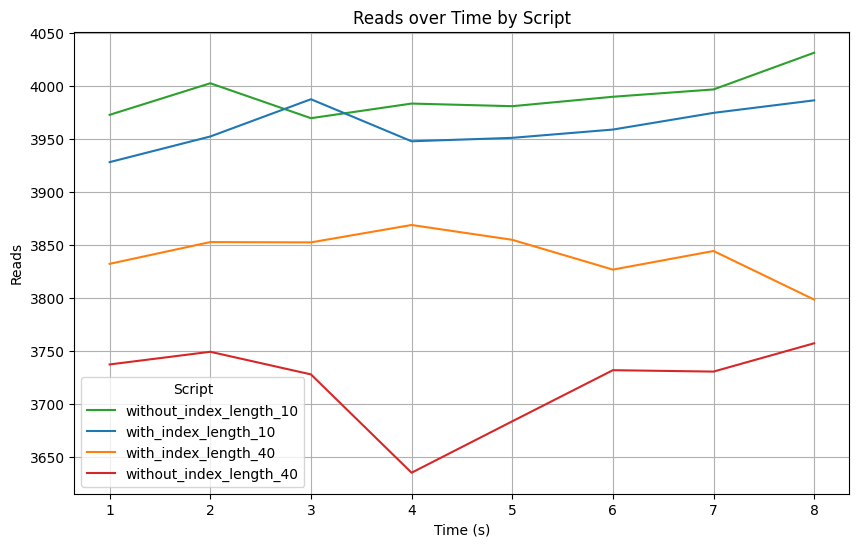
\includegraphics[width=\textwidth]{PNGs/Script/Index/B_Tree/low-count/Reads}
        \caption{Mit 10 und 40 Datensätze}
        \label{indexing-b-tree-low-reads}
    \end{subfigure}
    \hfill
    \begin{subfigure}[t]{0.48\textwidth}
        \centering
        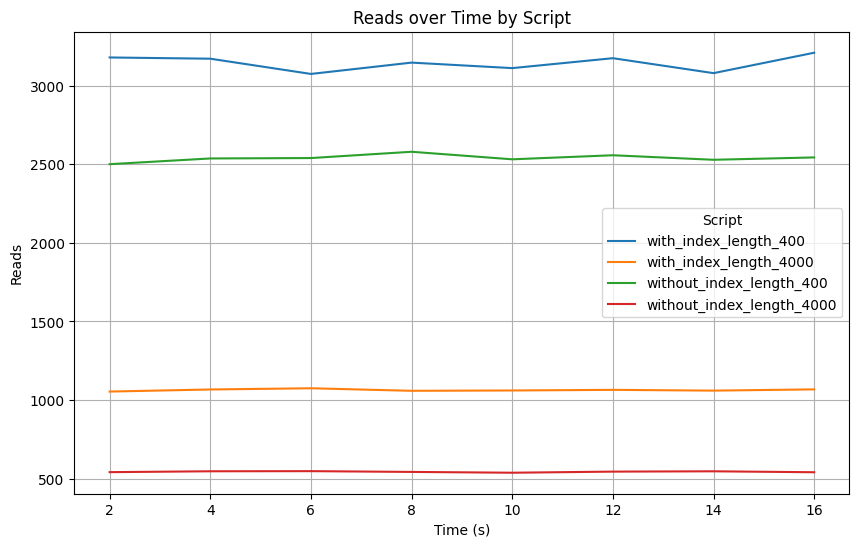
\includegraphics[width=\textwidth]{PNGs/Script/Index/B_Tree/high-count/Reads}
        \caption{Mit 400 und 4000 Zeilen}
        \label{indexing-b-tree-high-reads}
    \end{subfigure}
    \vspace{-6pt}
    \caption[B-Tree-Indexing: Mit Index vs Ohne]{Grafik zeigt Performance mit und ohne Index für Readsabfragen}
    \label{fig:indexing-vs-no}
\end{figure}
\vspace{-15pt}

In der Abbildung~\ref{indexing-b-tree-low-reads} ist zu erkennen, dass bei 10 Datensätzen die Kundentabelle ohne Indizes schneller ist als die mit Indizes.
Bei 40, 400 oder 4000 Zeilen (siehe~\ref{indexing-b-tree-low-reads} und~\ref{indexing-b-tree-high-reads}) wird die Wirkung der Indizes deutlich.
Der Unterschied bei 40 Datensätzen ist zwar etwas geringer, aber in den anderen Fällen sind die Unterschiede noch größer.
Interessant ist, dass es nicht linear oder quadratisch mit der Anzahl an Datensätzen in der Tabelle steigt, sondern bei 400 und 4000 Zeilen beträgt der Unterschied zur Tabelle ohne Index jeweils etwa 500--700 Abfragen.
Bei der Schreibgeschwindigkeit liegen beide auf einem sehr ähnlichen Niveau, wobei die Version ohne Index tendenziell einen leichten Vorteil hat.

Mit dem vorherigen Benchmark können die Vorteile eines Indexes bereits deutlich erkannt werden.
Nun soll jedoch auch die Funktionalität des B-Tree-Indexes in Bezug auf unterschiedliche Selects untersucht werden.
Dazu wird erneut die Kundentabelle erstellt, aber diesmal wird nur ein Index definiert (siehe~\ref{lst:indexing-create-combined}).
Anschließend wird die Tabelle mit einer festgelegten Anzahl an Datensätzen befüllt und es werden unterschiedliche Select-Befehle ausgeführt.
Im Codeblock~\ref{lst:indexing-b-tree-selects} sind aus Platzgründen nur die Where-Bedingungen zu sehen und am Ende jeder Zeile steht der Name der Query, damit später in der Analyse nachvollzogen werden kann, welche Query welche Performance liefert.

\vspace{-5pt}
\begin{lstlisting}[language=SQL,caption=Unterschiedliche Where-Bedingungen für B-Tree-Index,label={lst:indexing-b-tree-selects},basicstyle=\ttfamily\scriptsize]
WHERE NAME LIKE 'M%'; -- columm_prefix
WHERE NAME = 'Müller' AND VORNAME = 'Max' AND GEBURTSTAG < '1980-01-01'; -- combined_match_with_range
WHERE NAME = 'Müller' AND VORNAME LIKE 'M%' ORDER BY GEBURTSTAG; -- exact_with_prefix
WHERE NAME = 'Müller' AND VORNAME = 'Max' AND GEBURTSTAG = '1960-01-01'; -- full_match
WHERE NAME = 'Müller'; -- leftmost_prefix
WHERE GEBURTSTAG < '1980-01-01'; -- not_leftmost
WHERE NAME BETWEEN 'Müller' AND 'Schulz'; -- range_values
WHERE NAME = 'Müller' AND VORNAME LIKE 'M%' AND GEBURTSTAG < '1980-01-01'; -- range_with_like
WHERE NAME = 'Müller' AND GEBURTSTAG < '1980-01-01'; -- skip_columns
\end{lstlisting}
\vspace{-5pt}

Anhand der Grafik in Abbildung~\ref{fig:indexing-b-tree-query-reads} lässt sich erkennen, bei welchen Abfragen der Index am effizientesten ist.
Auf der linken Seite können die Ergebnisse für die Read-Befehle mit Index betrachtet werden, während auf der rechten Seite die Werte ohne Index zu sehen sind.

\vspace{-8pt}
\begin{figure}[H]
    \centering
    \begin{subfigure}[t]{0.48\textwidth}
        \centering
        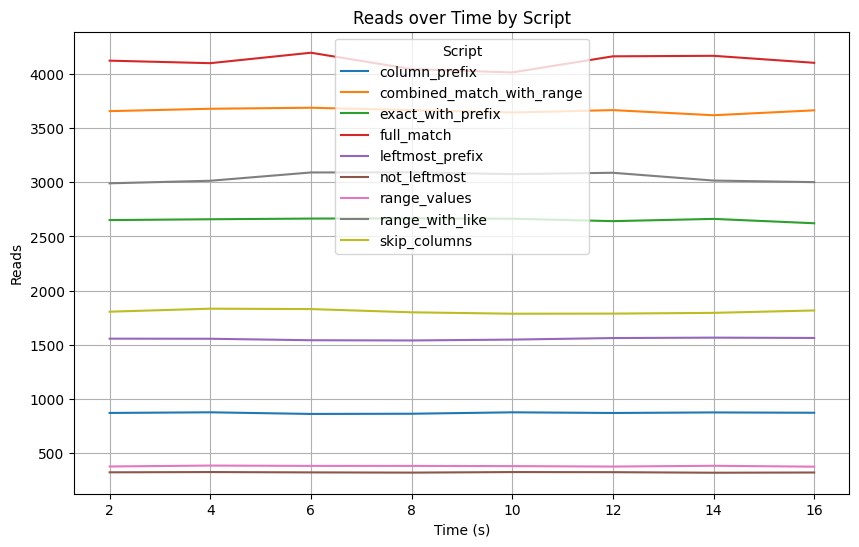
\includegraphics[width=\textwidth]{PNGs/Script/Index/B_Tree/b-tree-query-differences/Reads}
        \caption{Mit Index}
        \label{indexing-b-tree-query-reads-index}
    \end{subfigure}
    \hfill
    \begin{subfigure}[t]{0.48\textwidth}
        \centering
        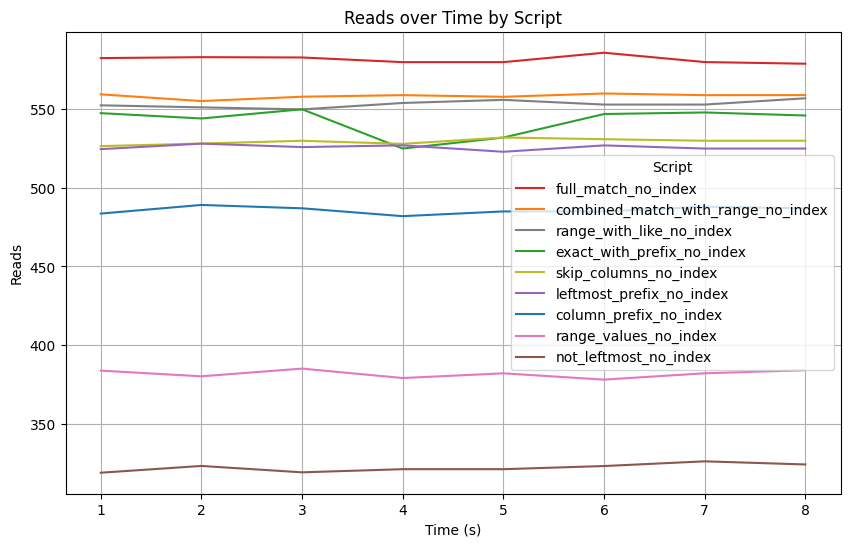
\includegraphics[width=\textwidth]{PNGs/Script/Index/B_Tree/b-tree-query-differences-no-index/Reads}
        \caption{Ohne Index}
        \label{indexing-b-tree-query-reads-no-index}
    \end{subfigure}
    \vspace{-5pt}
    \caption[B-Tree-Indexing: Unterschiedliche Selects mit Index und Ohne]{Visualisierung von unterschiedlichen Select-Queries mit und ohne Index}
    \label{fig:indexing-b-tree-query-reads}
\end{figure}
\vspace{-15pt}

Zunächst fällt auf, dass die Reihenfolge für die Werte mit und ohne Index komplett identisch ist.
Dies ist direkt erkennbar, da die Legenden beider Grafiken nach dem durchschnittlichen Wert über die gesamte Zeit sortiert sind.
Damit die richtigen Schlüsse aus der Grafik gezogen werden können, muss zunächst ermittelt werden, wie viele Zeilen die unterschiedlichen Queries zurückgeben.
Dazu werden die Abfragen zusätzlich mit dem \texttt{COUNT(*)}-Operator durchgeführt und die Ergebnisse in die Log-Datei geschrieben.
Anschließend werden die Werte entnommen und in einer Tabelle zusammengefasst.

\vspace{-5pt}
\begin{table}[H]
    \centering
    \scriptsize
    \begin{tabular}{|l|l|l|l|}
        \hline
        \textbf{Select-Query} & \textbf{Anzahl an Zeilen} & \textbf{Faktor} & \textbf{Index benutzt?} \\
        \hline
        full\_match & 0 & 7.31 & ja \\
        combined\_match\_with\_range & 8 & 6.75 & ja \\
        range\_with\_like & 29 & 5.80 & ja \\
        exact\_with\_prefix & 51 & 5.03 & ja \\
        skip\_columns & 146 & 3.77 & ja \\
        leftmost\_prefix & 255 & 3.13 & ja \\
        column\_prefix & 517 & 1.88 & ja \\
        range\_values & 1340 & 1.00 & nein \\
        not\_leftmost & 2371 & 1.02 & nein \\
        \hline
    \end{tabular}
    \vspace{3pt}
    \caption{Ergebnisse der COUNT(*)-Abfragen für B-Tree-Index}
    \label{tab:indexing_b_tree_count_results}
\end{table}
\vspace{-30pt}

Anhand der Spalte \texttt{Anzahl an Zeilen} lässt sich erkennen, dass die Queries, die am wenigsten Zeilen zurückgeben, auch diejenigen sind, bei denen die höchste Performance erzielt wird.
Damit ist auch die Reihenfolge mit und ohne Index gleich, weshalb man meinen könnte, dass der Index keinen Einfluss auf die Performance hat.
Dies betrifft jedoch nur die Reihenfolge, nicht aber die Werte der Abfragen, da hier deutliche Unterschiede erkennbar sind.
Anschaulich wird das mit der Betrachtung der Spalte \texttt{Faktor}.
Um den Wert zu berechnen, werden die Werte aus der Gesamtstatistik entnommen und die Version mit Index durch die Version ohne Index geteilt.
Dadurch lässt sich erkennen, dass \texttt{full\_match} zwar bei beiden Versionen am schnellsten ist, jedoch mit Index etwa 7-mal schneller als ohne.
Es lässt sich auch erkennen, dass je weniger Zeilen zurückgegeben werden, desto größer ist der Faktor.
Bei den Queries \texttt{range\_values} und \texttt{not\_leftmost} liegt der Faktor sehr nah 1, was bedeutet, dass der Index keinen Einfluss auf die Performance hat.
Deshalb stellt sich auch die Frage, ob der Index überhaupt verwendet wird.
Um das zu überprüfen, wird der \texttt{EXPLAIN}-Operator verwendet, das Ergebnis erneut geloggt und der Tabelle hinzugefügt.
Und tatsächlich sehen wir, dass die vermuteten Queries die einzigen sind, bei denen der Index nicht verwendet wird.

\section{Hash-Index}\label{sec:indexing-hash-index}
Ein weiterer Indextyp, der betrachtet wird, ist der Hash-Index.
Dieser basiert auf einer Hash-Tabelle und ist daher nur für exakte Suchanfragen geeignet, die alle Spalten des Indexes verwenden.
In MySQL unterstützt nur die Memory-Storage-Engine explizite Hash-Indizes.
Einige Storage-Engines, wie zum Beispiel InnoDB, können erkennen, wenn bestimmte Index-Werte besonders häufig abgefragt werden.
Sie erstellen dann automatisch einen Hash-Index für diese Werte im Speicher, der zusätzlich zu den bestehenden B-Baum-Indizes genutzt wird.
Die Funktionsweise der Storage-Engine lässt sich wie folgt beschreiben.

Für jede Zeile wird mithilfe einer Hash-Funktion ein Hash-Wert der indexierten Spalte berechnet.
Der Hash-Wert (engl.\ hash code) ist eine kleine Zahl, die sich in der Regel von den Hash-Werten anderer Zeilen unterscheidet.
Anschließend wird die Position im Index gesucht und man findet einen Zeiger auf die entsprechende Zeile.
In letzten Schritt überprüft man die Werte der Zeile, um sicherzustellen, dass es sich um die richtige Zeile handelt.

Wenn mehrere Werte denselben Hash-Wert besitzen, speichert der Index die Zeiger auf die Zeilen (engl.\ row pointers) in demselben Hash-Tabelleneintrag, typischerweise mithilfe einer verketteten Liste (z.B.\ einer Linked List).
Hash-Kollisionen können die Leistung eines Hash-Index beeinträchtigen, da jeder Zeiger in der verketteten Liste durchlaufen und die entsprechenden Werte mit dem Suchwert verglichen werden müssen, um die richtigen Zeilen zu finden.
Das ist auch bei Index-Wartungsoperationen mit viel Aufwand verbunden.
Es gibt auch eindeutige Hash-Indizes, die stellen sicher, dass für jeden Hash-Wert nur ein einziger Eintrag existiert.
Bei Konflikten wird ein Mechanismus wie die Open Addressing-Strategie (z.B.\ Linear Probing) eingesetzt, um Konflikte zu lösen und den Speicherplatz effizient zu verwalten.
Hierbei wird versucht, Konflikte direkt innerhalb der Hash-Tabelle zu bewältigen, anstatt auf zusätzliche Datenstrukturen wie verkettete Listen zurückzugreifen.
Jedoch werden die eindeutigen Hash-Indizes nicht von der Memory-Engine in MySQL unterstützt.

%Um die Verwendung des Hash-Indexes zu veranschaulichen, benutzen folgt folgendes Beispiel:
%
%\vspace{-5pt}
%\begin{lstlisting}[language=SQL]
%SELECT * FROM KUNDEN WHERE NAME = 'Peter';
%\end{lstlisting}
%\vspace{-8pt}
%
%Zunächst berechnet MySQL den Hash-Wert für \texttt{'Peter'} und verwendet diesen, um den entsprechenden Zeiger im Index zu finden.
%Angenommen, die Hash-Funktion liefert für \texttt{'Peter'} den Wert \texttt{7654}.
%In diesem Fall sucht MySQL im Index an der Position 7654 und findet einen Zeiger auf Zeile 3.
%Im letzten Schritt wird der Wert in Zeile 3 mit \texttt{'Peter'} verglichen.
%Da die Indizes nur kompakte Hash-Werte speichern, sind Hash-Indizes äußerst platzsparend und Suchvorgänge erfolgen in hoher Geschwindigkeit.

Ähnlich wie der B-Baum-Index hat aber auch der Hash-Index einige Einschränkungen.
Zum einen enthält der Index nur Hash-Werte und Zeiger auf Zeilen (engl.\ row pointers), jedoch nicht die Werte selbst.
Deshalb kann MySQL den Index nicht verwenden, um das Einlesen der Zeilen zu vermeiden.
Zum anderen können Hash-Indizes, anders als B-Baum-Indizes, nicht für Sortierungen verwendet werden, da die Werte nicht in einer geordneten Reihenfolge gespeichert sind.
Darüber hinaus ermöglichen Hash-Indizes keine partiellen Schlüsselübereinstimmungen, da der Hash-Wert aus dem gesamten indexierten Wert berechnet wird.
Bei einem Index aus den Spalten (A, B) und einer \texttt{WHERE}-Klausel, die nur auf A verweist, ist dies daher nicht hilfreich.
Ein weiterer Nachteil von Hash-Indizes ist, dass sie keine Bereichsabfragen unterstützen und nur für Gleichheitsvergleiche wie \texttt{=}, \texttt{<=>} und \texttt{IN()} geeignet sind.

Als Nächstes werden die Benchmarks mit Hash-Indizes betrachtet.
Dazu wird erneut die Kundentabelle verwendet und diesmal nur ein Index für die Spalte \texttt{NAME} erstellt.
Am Ende des \texttt{CREATE INDEX}-Befehls muss \texttt{USING HASH} hinzugefügt werden, damit statt des standardmäßigen B-Tree-Index der Hash-Index verwendet wird.
Danach befüllen wieder die Tabelle mit Testdaten.
Diesmal wird beim ersten Benchmark der Einfluss von Hash-Kollisionen auf die Performance untersucht.
Um den Grad der Kollisionen zu verändern, wird eine Variable verwendet, die die obere Grenze für die zufällige Generierung einer Zahl darstellt.
Anschließend werden alle Zeilen mit dem Wert \texttt{Kunde\_1} für die Spalte \texttt{NAME} abgefragt und die Tests werden mit den Kollisionswahrscheinlichkeiten von 25\%, 10\%, 5\% und 1\% durchgeführt.

\vspace{-4pt}
\begin{figure}[H]
    \centering
    \begin{subfigure}[t]{0.48\textwidth}
        \centering
        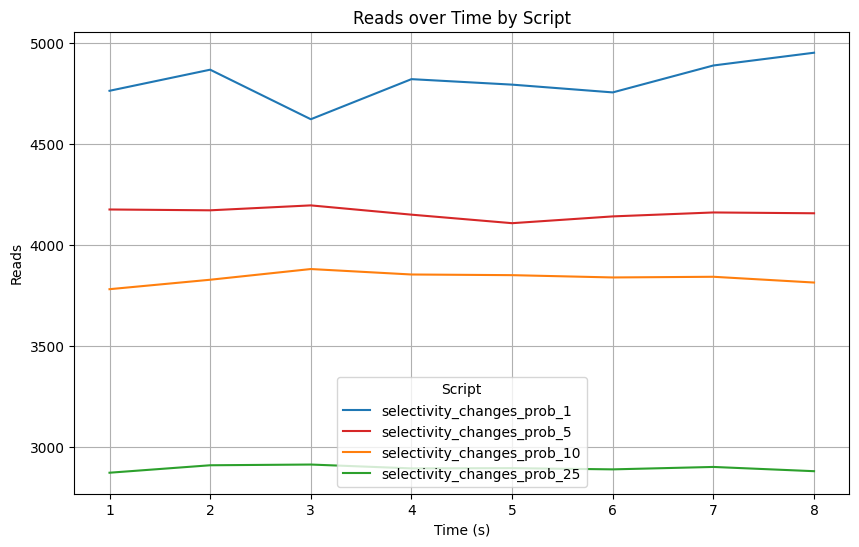
\includegraphics[width=\textwidth]{PNGs/Script/Index/Hash/hash-selectivity-change/Reads}
    \end{subfigure}
    \hfill
    \begin{subfigure}[t]{0.48\textwidth}
        \centering
        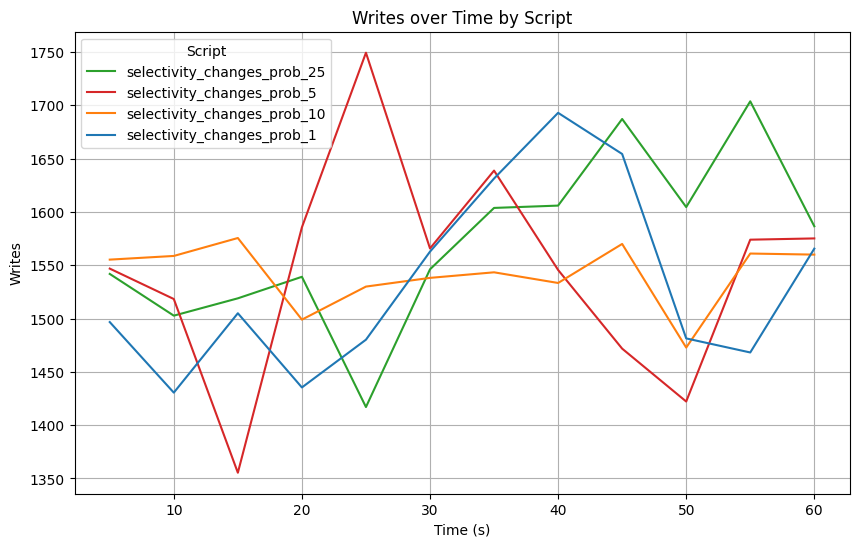
\includegraphics[width=\textwidth]{PNGs/Script/Index/Hash/hash-selectivity-change/Writes}
    \end{subfigure}
    \vspace{-8pt}
    \caption[Hash-Indexing: Auswirkungen von Hashkollisionen]{Vergleich der Auswirkungen von Hashkollisionen}
    \label{fig:hash-collision-comparison}
\end{figure}
\vspace{-17pt}

An den Ergebnissen in Abbildung~\ref{fig:hash-collision-comparison} ist zu erkennen, dass je geringer die Wahrscheinlichkeit für eine Kollision ist, desto schneller fällt die Select-Abfrage aus.
Es fällt auch auf, dass die Unterschiede zwischen den verschiedenen Kollisionswahrscheinlichkeiten sehr groß sind.
Hingegen die Einfüge-Performance ist bei allen 4 Varianten auf einem ähnlichen Niveau.
Als zweiten Test soll überprüft werden, ob der Index bei bestimmten Select-Queries benutzt wird oder nicht.
Dazu wird erneut die Kundentabelle verwendet, der gleiche Index wie in Beispiel~\ref{lst:indexing-create-combined} erstellt, die Testdaten eingefügt und die Select-Befehle aus~\ref{lst:indexing-b-tree-selects} genutzt.
Dieses Mal werden aber nicht alle Select-Befehle verwendet, sondern nur die aus folgender Tabelle:

\vspace{-4pt}
\begin{table}[H]
    \centering
    \scriptsize
    \begin{tabular}{|l|l|l|l|}
        \hline
        \textbf{Select-Query} & \textbf{Anzahl an Zeilen} & \textbf{Faktor} & \textbf{Index benutzt?} \\
        \hline
        full\_match & 0 & 2.96 & ja \\
        combined\_match\_with\_range & 9 & 1.16 & nein \\
        exact\_with\_prefix & 42 & 1.13 & nein \\
        leftmost\_prefix & 204 & 1.22 & nein \\
        \hline
    \end{tabular}
    \vspace{3pt}
    \caption{Ergebnisse der COUNT(*)-Abfragen für Hash-Index}
    \label{tab:indexing_hash_count_results}
\end{table}
\vspace{-30pt}

Anhand der Spalten \texttt{Faktor} und \texttt{Index benutzt?} kann erkannt werden, dass der Index nur bei der \texttt{full\_match}-Abfrage benutzt wird.
Das stimmt auch mit den Ergebnissen aus der Abbildung~\ref{fig:indexing-hash-query-reads} überein, da ohne Index alle Abfragen auch einem ähnlichen Niveau liegen, aber mit Index sticht eine deutlich hervor.
Interessant ist, dass die Query mit 206 zurückgegebenen Zeilen nur unwesentlich langsamer ist als die anderen.
Die Reihenfolge ist wieder bei beiden identisch und hängt von der Anzahl der zurückgegebenen Zeilen ab.

\vspace{-8pt}
\begin{figure}[H]
    \centering
    \begin{subfigure}[t]{0.48\textwidth}
        \centering
        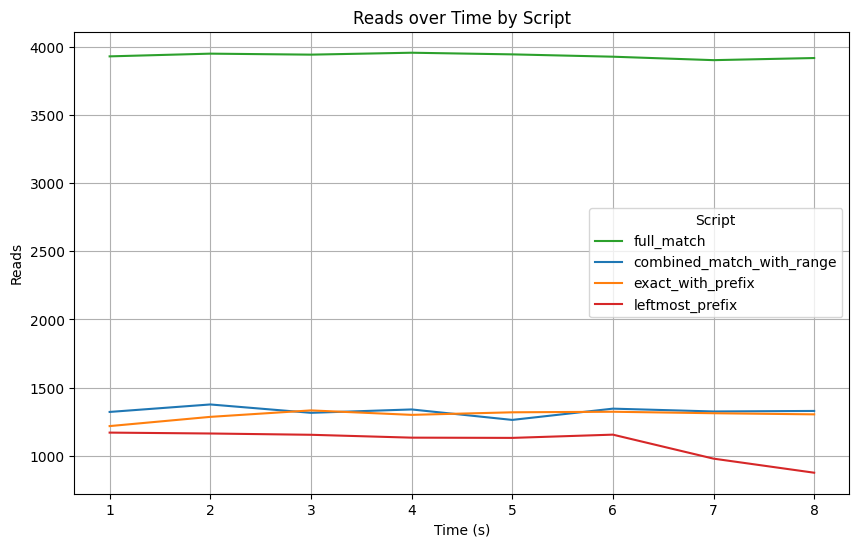
\includegraphics[width=\textwidth]{PNGs/Script/Index/Hash/hash-query-differences/Reads}
    \end{subfigure}
    \hfill
    \begin{subfigure}[t]{0.48\textwidth}
        \centering
        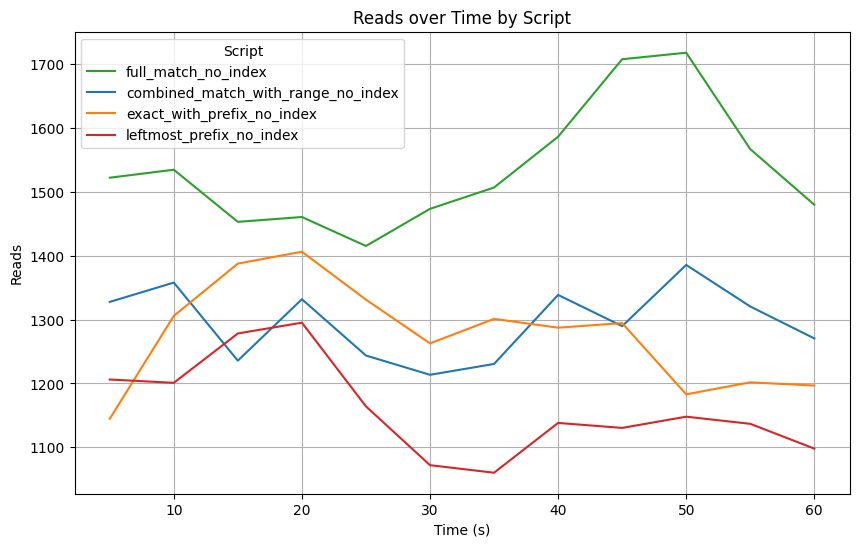
\includegraphics[width=\textwidth]{PNGs/Script/Index/Hash/hash-query-differences-no-index/Reads}
    \end{subfigure}
    \vspace{-8pt}
    \caption[Hash-Indexing: Unterschiedliche Abfragen mit Index und Ohne]{Grafik visualisiert Select-Queries mit (links) und ohne (rechts) Index}
    \label{fig:indexing-hash-query-reads}
\end{figure}

\section{Vergleich zwischen B-Tree- und Hash-Index}\label{sec:indexing-comp-b-tree-hash-index}

In den vorherigen Kapiteln wurden der B-Tree-Index und der Hash-Index jeweils getrennt voneinander betrachtet.
Dabei wurde auch analysiert, bei welchen Select-Queries die Indizes Vorteile bieten und bei welchen nicht.
Damit fehlt noch der Vergleich zwischen B-Tree- und Hash-Index.

Um die Unterschiede zwischen beiden Indexstrukturen genauer zu analysieren, wird ein neuer Benchmark durchgeführt, der die Skripte aus Kapitel~\ref{sec:indexing-b-baum-index} und~\ref{sec:indexing-hash-index} wiederverwendet.
Da der Hash-Index aber nur 4 unterschiedliche Select-Queries aufruft, sollen auch nur diese mit dem B-Tree-Index ausgeführt werden.
Dazu wird einfach der Parameter~\texttt{selects} beim Aufruf des Orchestrator-Skripts hinzugefügt und das Skript anschließend ausgeführt.

\vspace{-4pt}
\begin{figure}[H]
    \centering
    \begin{subfigure}[t]{0.48\textwidth}
        \centering
        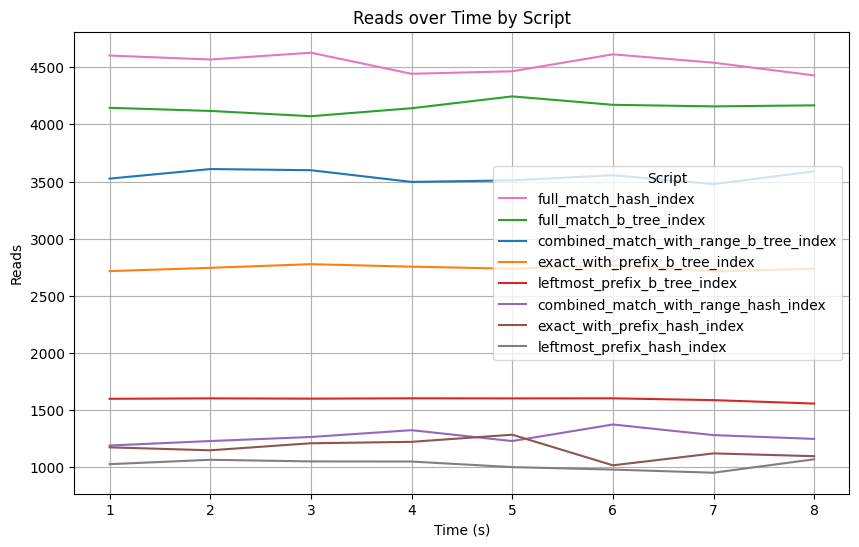
\includegraphics[width=\textwidth]{PNGs/Script/Index/B_Tree/hash-vs-b-tree-comparison/Reads}
        \caption{Anzahl der Lesezugriffe}
        \label{indexing-hash-vs-b-tree-comparison-reads}
    \end{subfigure}
    \hfill
    \begin{subfigure}[t]{0.48\textwidth}
        \centering
        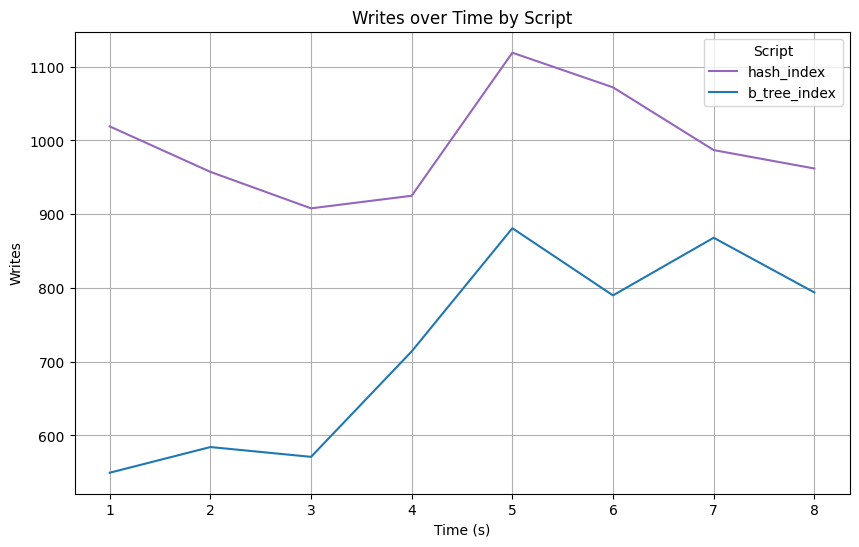
\includegraphics[width=\textwidth]{PNGs/Script/Index/B_Tree/hash-vs-b-tree-comparison/Writes}
        \caption{Anzahl der Schreibzugriffe}
        \label{indexing-hash-vs-b-tree-comparison-writes}
    \end{subfigure}
    \vspace{-2pt}
    \caption[Indexing: Vergleich von B-Tree- und Hash-Index]{Vergleich der Select-Query-Performance von B-Tree- und Hash-Index}
    \label{fig:indexing-hash-b-tree-comp}
\end{figure}
\vspace{-12pt}

In der Abbildung~\ref{indexing-hash-vs-b-tree-comparison-reads} sehen die Performance für die unterschiedlichen Select-Befehle.
Die höchste Transaktionsrate erzielt der Hash-Index, sofern der vollständige Schlüssel angegeben wird (\texttt{full\_match}).
Dicht darauf folgt der B-Tree-Index mit derselben Abfrage, allerdings mit etwa 10\% weniger Zugriffen.
Bei den übrigen Abfragen schneidet hingegen der B-Tree-Index deutlich besser ab, in einigen Fällen sogar bis zu dreimal schneller als der Hash-Index.
Der Grund dafür ist bereits aus den anderen Kapiteln bekannt.
Da der Hash-Index nur bei exaktem Schlüsselabgleich zum Einsatz kommt, wird er bei den anderen Abfragen nicht verwendet.
Mithilfe des \texttt{EXPLAIN}-Operators wurde festgestellt, dass stattdessen der B-Tree-Index verwendet wird, was die starken Unterschiede erklärt.

Betrachtet man die Schreibperformance (Abbildung~\ref{indexing-hash-vs-b-tree-comparison-writes}), zeigt sich, dass der Hash-Index etwa 30--40\% schneller ist als der B-Tree-Index.
Wenn eine Anwendung also eine hohe Schreiblast hat, könnte der Hash-Index eine bessere Wahl sein, da er weniger Mehraufwand verursacht.
Zusammenfassend lässt sich festhalten, dass der Hash-Index einen leichten Vorteil hat, wenn beide Indexe greifen.
Andernfalls überwiegen die Stärken des B-Tree-Indexes.
